\chapter{Synchronisatie}
\label{hoofdstuk:synchronisatie}
Het thera project bestaat al een tijdje en er zijn reeds vele XML-bestanden met validaties van voorstellen in omloop. Ondanks de eventuele overgang van het oude naar het nieuwe systeem is het belangrijk dat deze resultaten niet verloren gaan, het heeft immers veel werk gekost om ze te maken. Als bestanden verschillende paren bevatten --- omdat ze bijvoorbeeld door een ander identificatiealgoritme zijn gegenereerd --- maar over eenzelfde opgraving gaan, is het ook nuttig om deze te consolideren. Indien er geen internetverbinding is of even geen storing van anderen wil hebben, kan een lokale kopie ge\"extraheerd en later terug ge\"importeerd worden. Dit alles kan gedaan worden met de synchronisatiecomponenten van dit project.

\section{Opzet}
Om te synchroniseren selecteert men een meester- en een slaaf-database, de conventie is dat de slaaf door de meester zal geabsorbeerd worden. Na het proces heeft de meester alle gewenste veranderingen en blijft de slaaf onveranderd over. Er zijn verschillende fasen (voorlopig 3): \textbf{Gebruikers}, \textbf{Paren} en \textbf{Attributen}. In elke fase krijgt de gebruiker een scherm te zien met daarin de verschillen tussen beide databases, het biedt de mogelijkheid om aanpassingen te maken alvorens naar de volgende stap te gaan. Het is belangrijk gebruikers keuzes te laten maken waarin ze ge\"interesseerd zijn en ze niet lastig te vallen met keuzes die ze niet willen maken, beide zaken negeren leidt tot frustraties~\cite{Joel2001}. De algoritmes proberen daarom steeds een standaardkeuze in te vullen aan de hand van heuristieken, deze kunnen indien gewenst verworpen worden. Als er door gebrek aan informatie geen automatische belissing kan genomen worden, moeten alle conflicten eerst manueel opgelost worden. Figuren~\ref{fig:merge-attrib} en~\ref{fig:merge-choose} tonen hoe deze stappen eruitzien en figuur~\ref{fig:merging-overview} geeft een schematische kijk op het systeem. Sommige SQL-implementaties bieden automatische replicatie aan, dit wordt niet gebruikt omdat het minder flexibel is qua conflictresolutie noch compatibel over implementaties heen.\\

\begin{figure}[ht]
	\begin{center}
		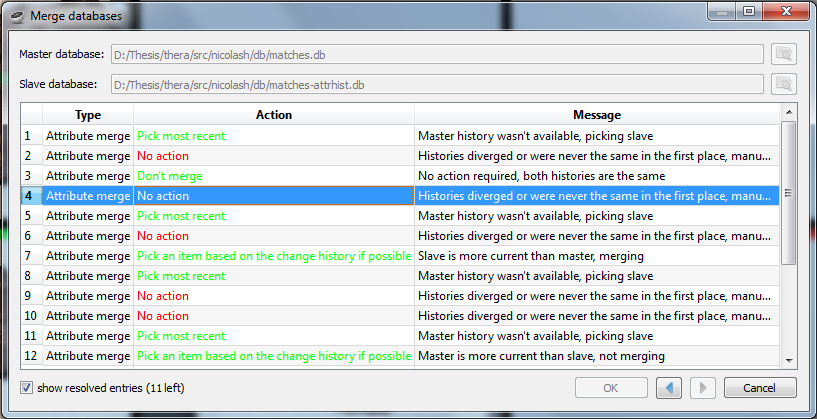
\includegraphics[width=1.0\columnwidth]{images/merge-action-1-small.png}
		\caption{Een uittreksel van de attributen-fase van het synchronisatieproces. ``No Action''  duidt aan dat er geen automatische resolutie toegepast is geweest, hierop dubbelklikken geeft een keuzescherm weer (rechts).}
		\label{fig:merge-attrib}
	\end{center}
\end{figure}

\begin{figure}[ht]
	\begin{center}
		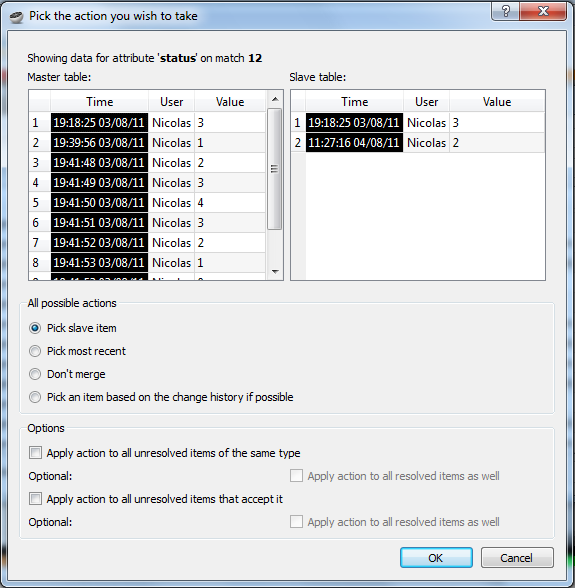
\includegraphics[width=0.5\columnwidth]{images/merge-action-2-small.png}
		\caption{Elk type conflict laat een aantal manieren toe om het op te lossen. Deze figuur beeldt een attribuut-conflict voor.}
		\label{fig:merge-choose}
	\end{center}
\end{figure}

% Het gros van het onderzoek op het vlak van samenvoegingsalgoritmen gaat over het combineren van tekstbestanden, hier werden reeds vele innovatieve aanpakken voor ontwikkeld\footnote{Arbitraire tekst is moeilijk to synchroniseren omwille van de vele vrijheidsgraden, een tekstbestand kan op ontelbare manieren veranderen en het is niet steeds triviaal om te zien hoe twee conflicterende aanpassingen in elkaar moeten gevoegd worden}. Gelukkig vallen vele problemen weg door de eenvoudigere (minder vrije) structuur van de data in dit project. Voor de attributen wordt een geschiedenis bijgehouden. De algoritmen gebruikt voor elke fase worden in de volgende secties uit de doeken gedaan.

\subsection{Paren}
In deze stap worden de voorstellen zonder attributen uit beide databases vergeleken en gesynchroniseerd. Deze objecten bevatten een identificatiecode, twee namen van fragmenten en een 3D-transformatiematrix. De identificatiecode is echter geen uniek gegeven over alle databases, eerder een manier om effici\"ent naar het object te verwijzen binnen eenzelfde database. Het is echter duidelijk dat als twee voorstellen uit dezelfde fragmenten bestaan en dezelfde transformatie hebben, ze identiek kunnen geacht worden. De aanwezigheid van afrondingsfouten en duplicaten is problematisch. Duplicaten zullen per definitie een gelijkaardige transformatiematrix hebben, hoe ze te onderscheiden van afrondingsfouten? De matrix van een voorstel uit de slaaf-database wordt afgetrokken van de matrix van elk voorstel uit de meester-database dat uit dezelfde fragmenten bestaat, hiervan wordt vervolgens de Frobenius norm\footnote{De euclidische norm van de vector die ontstaat als men de rijen of kolommen van een matrix achter elkaar plaatst.} genomen. Hieruit ontstaat een rij van getallen die aangeven hoe gelijkaardig het voorstel is aan elk van de mogelijke overeenkomstige voorstellen uit de meester-database. Het kleinste getal geeft het meest overeenkomstige paar aan. Indien dit kleinste getal een ordegrootte (10x) kleiner is dan het maximale verschil tussen dit overeenkomstig paar en diens duplicaten, wordt aangenomen dat de paren in kwestie identiek zijn. Indien niet wordt het paar uit de slaaf-database als een nieuwe paar ingevoerd.\\

De volledige voorstellenlijst van beide databases moet dus nagekeken worden. Eenmaal beiden in het geheugen geladen zijn verloopt het vergelijkingsproces vrij snel (er wordt een hashmap aangemaakt om in constante tijd te kunnen zien welke voorstellen uit dezelfde fragmenten bestaan). Dit wil natuurlijk wel zeggen dat het synchroniseren van pure paren op zich over het internet niet werkbaar is met een database van miljoenen elementen. Gelukkig gebeurt het niet vaak dat onderzoekers paren toevoegen.\\

Paren die overeenkomen worden aan een identiteitsvertaler toegevoegd, waardoor latere fasen weten dat twee verschillende identificatienummers naar hetzelfde object verwijzen. Een paar dat niet gevonden werd in de meester-database wordt niet automatisch ingevoerd maar als een conflict weergegeven. De gebruiker kan gemakkelijk kiezen om dit toch te doen door ``assign new id'' als actie toe te kennen en aan te vinken om dit te doen voor alle gelijkaardige conflicten (zoals in figuur~\ref{fig:merge-choose}). Het alternatief is ``don't merge'', wat ervoor zorgt dat de nieuwe paren niet toegevoegd worden (en genegeerd in de volgende stappen).

\subsection{Attributen}
Het samenvoegen van attributen verloopt op een andere manier. Het is gemakkelijk te detecteren wanneer zich een conflict voordoet, namelijk als de waarden verschillen. Dit conflict oplossen gaat echter niet automatisch, als een \emph{commentaar}-attribuut bijvoorbeeld twee verschillende teksten bevat, welke is dan de juiste? Misschien de meest recente, zeker als blijkt dat een vorige waarde van de meest recente gelijk is aan de minder recente (gemeenschappelijk ouder). Om automatische resolutie te ondersteunen moet er dus een geschiedenislijst bijgehouden worden. Daarnaast kan nog gekeken worden naar de semantische inhoud van het attribuut om eventueel een oordeel te vellen als de geschiedenismethode faalt.

\subsubsection{Gemeenschappelijke ouder}
Indien beide databases voor een bepaald attribuut een stukje geschiedenis delen, is er een kans dat het conflict automatisch opgelost kan worden. Stel dat in een kopie van een database een attribuut verandert en ditzelfde attribuut is niet aangeraakt in de originele database. In dat geval kan de nieuwe waarde zonder meer overgenomen worden bij synchronisatie. Het kijken naar een gemeenschappelijke ouder om te synchronizeren wordt in de literatuur \emph{3-way merging}~\cite{sync:diff3} genoemd. De zojuist beschreven situatie komt overeen met het meest linkse vak in figuur~\ref{fig:okay-3-way}. Het is de meest voorkomende want uit de grote hoeveelheid paren is de kans klein dat exact dezelfde (in een korte tijdsspanne) bewerkt worden. In het geval dat dit wel zou gebeuren --- het middelste vakje in de figuur --- kan er niet op die manier gesynchroniseerd worden. Hetzelfde doet zich voor als de beide databases geen geschiedenis delen, deze situatie wordt voorgesteld door het meest rechtse vakje. Samenvattend kan er dus niet automatisch gehandeld worden als de geschiedenis divergeert.

\subsubsection{Context}
Toch zijn er situaties denkbaar waar er toch een oplossing is. Stel dat de validatiestatus van een bepaald voorstel ``niet geweten'' is en de database wordt gesplitst in database A en B. In database A wordt vervolgens de status op ``misschien'' gezet en in B op ``correct''. Als de synchronisatie afweet van de semantiek van statussen, zal het correct kunnen afleiden dat ``correct'' een krachtiger status is en dit verkiezen. Voor commentaren kan bijvoorbeeld gelden dat het meest recente de bovenhand krijgt. Dit zijn contextbeslissinggen, waarbij de component op de hoogte moet zijn van de betekenis achter de waarden. Dit soort acties kan over het algemeen niet overgezet worden van het \'ene attribuut op het andere, hetgeen aparte routines voor elk contextgevoelig attribuut veronderstelt.\\

Er zijn ook attributen waar dit soort beslissingen niet eenvoudig kunnen genomen worden (bvb. duplicaten), of waarvoor de routines nog niet gemaakt zijn. In dit laatste geval kan er geen automatische resolutie plaatsvinden en moet de gebruiker ingrijpen alvorens verder te gaan. Er zijn heel wat verschillende acties geldig op een attribuut conflict, enkele daarvan zijn: ``pick most recent'', ``prefer user [username]'', ``prefer slave'' en ``don't merge''.

\begin{figure}[ht]
	\begin{center}
		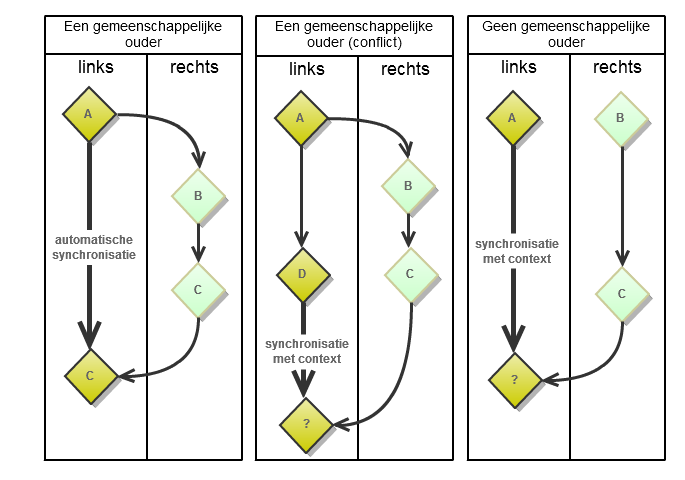
\includegraphics[width=1.0\columnwidth]{images/3-way-merge.png}
		\caption{Situaties waarin automatische resolutie gebaseerd op geschiedenis mogelijk is (eerste figuur) en waar contextinformatie nodig is (tweede en derde figuur). Links is hier gelijk aan de meester-database en rechts is de slaaf-database.}
		\label{fig:okay-3-way}
	\end{center}
\end{figure}

\subsection{Incrementele synchronisatie}
Omdat er een geschiedenis wordt bijgehouden is incrementele synchronisatie voor attributen mogelijk als beide databases geschiedenis delen. De geschiedenis wordt voor elk attribuut apart bijgehouden dus de gemakkelijkste en meest robuuste oplossing is om per attribuut een binair zoekalgoritme te laten zoeken naar het laatste gemeenschappelijke punt. In feite is dit hetzelfde algoritme als hetgene dat gebruikt wordt om de gemeenschappelijke ouder te vinden, met het verschil dat er in deze versie naar alle paren wordt gekeken in plaats van slechts \'e\'en. Dit is robuust omdat er veel verschillende manieren zijn om databases te kopi\"eren en er dus niet kan vertrouwd worden op het aanwezig zijn van splitindicatoren. Enkel de kost van het binair zoeken en het overzetten van de veranderde attributen is dan van belang. Op een database van 50000 paren kan dit een groot verschil opleveren als er bijvoorbeeld slechts 100 attributen veranderd zijn. Op die manier wordt synchroniseren over het internet mogelijk. 